
\input preamble.tex
\vskip 5pt

\vskip 5pt
\begin{center}
	\huge
	\textbf{Læringsoppdrag målesystemer for temperatur - Stasjon 11} \normalsize \vskip 5pt 
\end{center}

$$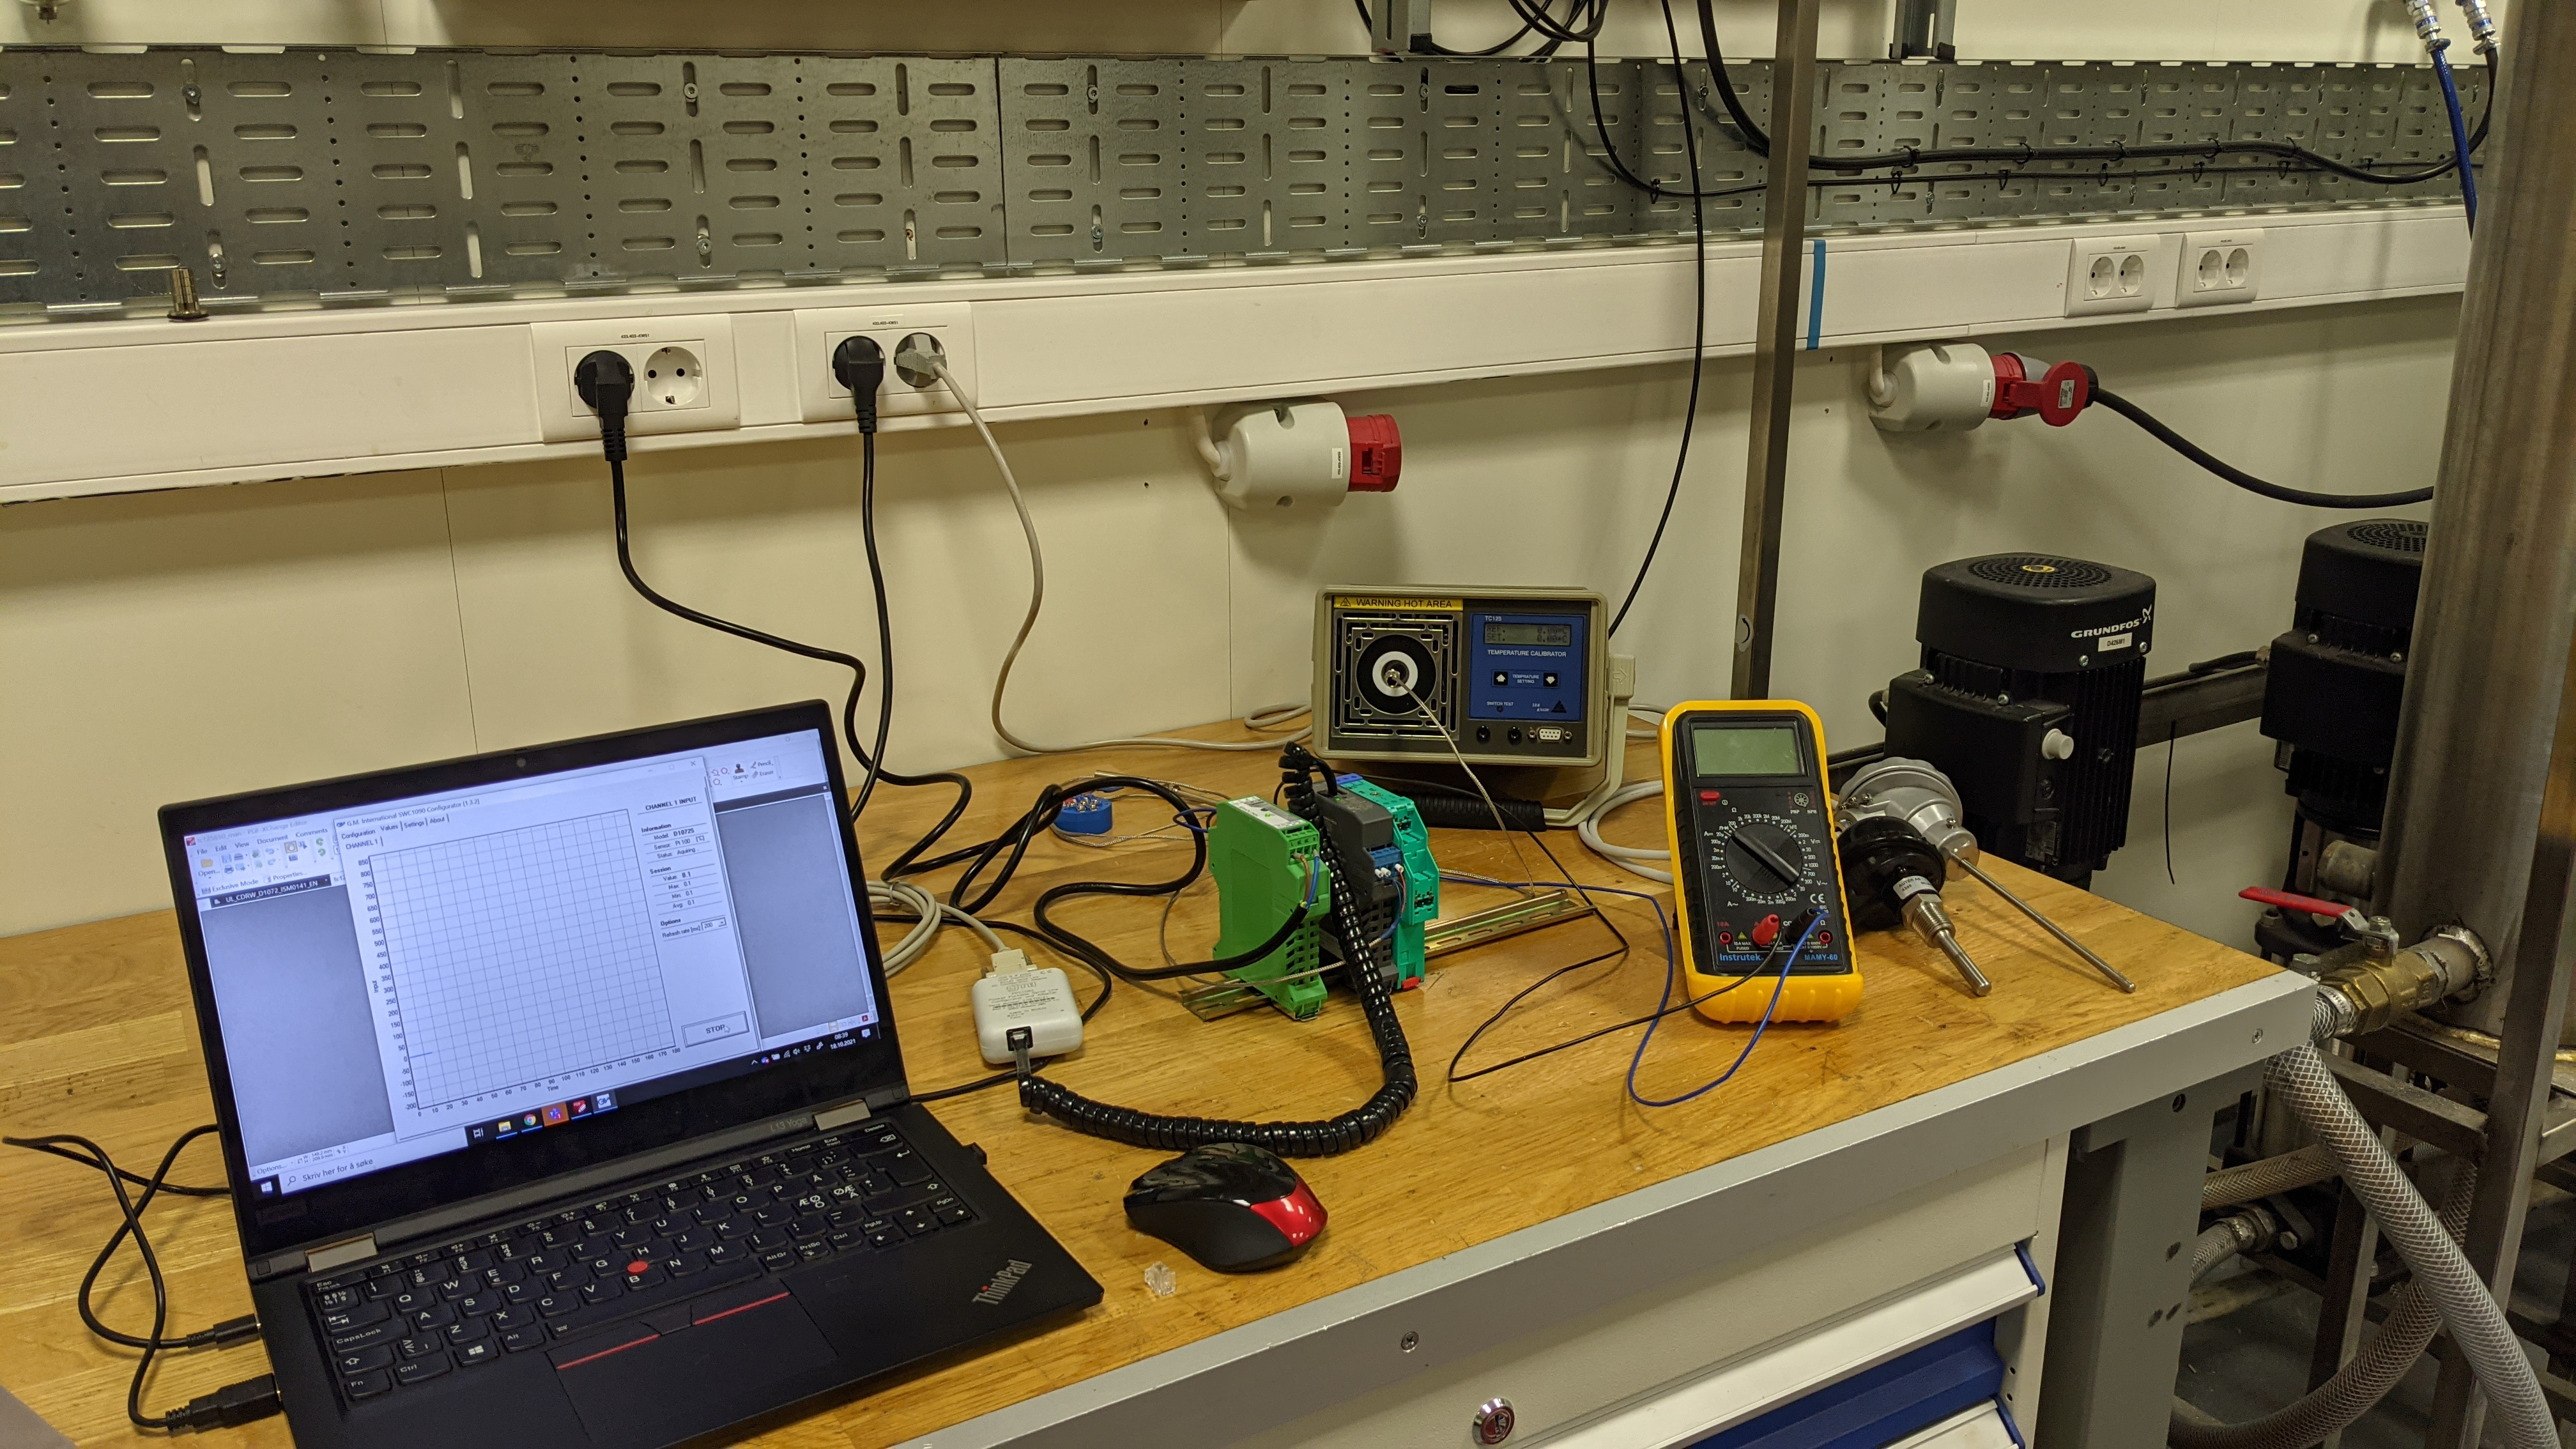
\includegraphics[width=13cm]{./lStasjon11x01.jpg}$$\\

\vskip 1cm
Dette læringsoppdraget består av følgende:

\begin{itemize}[noitemsep]
	\item Oppgavesett Temperaturregulering
	\item Arbeidsoppdrag målesystemer for temperatur
\end{itemize}


 
\vskip 5pt 

Du kan jobbe parallelt med alle oppgavene. 

\vskip 5pt 
\textbf{Bakgrunnsteori}
 I filen \href {https://autofaget.no/pdfs/afgv.pdf}{afgv.pdf} er følgende kapittler til hjelp for dette læringsoppdraget:
 \begin{itemize}[noitemsep]
	 \item Continuous temperature measurement
 \end{itemize}
\newpage
\textbf{Arbeidsoppdrag på stasjon11}

\vskip 1cm
\vskip 1cm
\textbf{Introdusjon}

\vskip 5pt 
I dette oppdraget skal du sette opp og kalibrere to målesystemer for temperatur. Det ene systemet skal benytte en transmitter fra GM (D1072S) og det andre en fra Pepperl+Fuchs (KFD2-UT2-Ex1). Begge disse transmitterne er laget for bruk i EX områder det skal vi ikke bry oss med i dette oppsraget. 
\\
Begge målesystemene må settes opp med software fra leverandøren:
\\
\textbf{Pepperl+Fuchs}
\\
For å programmere KFD2-UT2-Ex1, trenger du adapteren K-ADP-USB, samt programmet Pactware og Tilhørende DTM.
\\

Programvaren laster du ned her: 
\\
\href {https://www.pepperl-fuchs.com/norway/no/classid_163.htm?view=productdetails&prodid=83574#software}{PACTware 5.X}
\\
\href {https://www.pepperl-fuchs.com/norway/no/classid_1804.htm?view=productdetails&prodid=32802}{DTM Interface Technology}
\\
 

\href{https://files.pepperl-fuchs.com/webcat/navi/productInfo/doct/tdoct1599c_eng.pdf?v=20200320004907}{Veiledning} Installation and configuration guide Device Type Manager (DTM)
\\  
Eventuellt trenger du kanskje denne, men prøv først uten:
\\
\href {https://www.pepperl-fuchs.com/norway/no/classid_1805.htm?view=productdetails&prodid=27434}{Microsoft .NET}
\vskip 5pt 
\vskip 5pt 
\href {https://files.pepperl-fuchs.com/webcat/navi/productInfo/doct/tdoct0735e_eng.pdf?v=20200320004741}{Manual KFD-UT2-Ex1}

\vskip 5pt 

\textbf{GMI}
\\
Software til GMI D1072s finner du i mappen software vi bruker og verktøy (SWC1090.exe)
\\
Målesystemene skal ha følgende måleområder:
\begin{itemize}[noitemsep]
\item GMI 10-40°C
\item Pepperl+Fuchs -5-100°C
\end{itemize}

\vskip 5pt 

Det må fylles ut kalibreringssertifikat for begge målesystemene. 



\href {https://autofaget.no/temp/node2.html}{Leseoppgave}








\underbar{file i04841}
\vfil \eject
%(END_QUESTION)





%(BEGIN_ANSWER)


%(END_ANSWER)





%(BEGIN_NOTES)


%INDEX% Arbeisdoppdrag, Kompetanse, Nivå 1, Stasjonxx, Mal

%(END_NOTES)


\end{document}
